\documentclass[12pt,letterpaper,fleqn]{hmcpset}
\usepackage[margin=1in]{geometry}
\usepackage{graphicx}
\usepackage{amsmath,amssymb}
\usepackage{enumerate}
\usepackage{hyperref}
\usepackage{parskip}

\input{macros.tex}

% info for header block in upper right hand corner
\name{}
\class{Math189 SP20}
\assignment{Homework 5}
\duedate{Monday, Mar 2, 2019}

\begin{document}

Feel free to work with other students, but make sure you write up the homework
and code on your own (no copying homework \textit{or} code; no pair programming).
Feel free to ask students or instructors for help debugging code or whatever else,
though.

\begin{problem}[1]
\textbf{(Murphy 12.5 - Deriving the Residual Error for PCA)} It may be helpful to reference
section 12.2.2 of Murphy.
\begin{enumerate}[(a)]
    \item Prove that
        \[
            \left\|\xx_i - \sum_{j=1}^k z_{ij}\vv_j\right\|^2 = \xx_i^\T\xx_i - \sum_{j=1}^k\vv_j^\T \xx_i\xx_i^\T \vv_j.
        \]
        Hint: first consider the case when $k=2$. Use the fact that $\vv_i^\T\vv_j$ is 1 if $i=j$ and 0 otherwise.
        Recall that $z_{ij} = \xx_i^\T\vv_j$.

    \item Now show that
        \[
            J_k = \frac{1}{n}\sum_{i=1}^n \left(\xx_i^\T \xx_i - \sum_{j=1}^k\vv_j^\T \xx_i\xx_i^\T \vv_j\right) = \frac{1}{n}\sum_{i=1}^n \xx_i^\T\xx_i - \sum_{j=1}^k\lambda_j.
        \]
        Hint: recall that $\vv_j^\T \Sigmab \vv_j = \lambda_j\vv_j^\T\vv_j = \lambda_j$.

    \item If $k=d$ there is no truncation, so $J_d=0$. Use this to show that the error from only using $k<d$
        terms is given by
        \[
            J_k = \sum_{j=k+1}^d \lambda_j.
        \]
        Hint: partition the sum $\sum_{j=1}^d \lambda_j$ into $\sum_{j=1}^k \lambda_j$ and $\sum_{j=k+1}^d \lambda_j$.
\end{enumerate}
\end{problem}
\begin{solution}
    \begin{enumerate}[(a)]
        \item We have
            \begin{align*}
                (\xx_i - \sum_{j=1}^k z_{ij}\vv_j)^\T(\xx_i - \sum_{j=1}^k z_{ij}\vv_j) &= \xx_i^\T \xx_i - 2\sum_{j=1}^k z_{ij}\vv_j^\T\xx_i + \sum_{j=1}^K \vv_j^\T z_{ij}^\T  z_{ij} \vv_j \text{   (since $\vv_j \vv_j = 1$) } \\
                                                                                        &= \xx_i^\T \xx_i - 2\sum_{j=1}^k \xx_i^\T \vv_j\vv_j^\T\xx_i + \sum_{j=1}^k \vv_j^\T \xx_i \xx_i^\T \vv_j \text{   (since $\xx_i^\T \vv_j$ is a scalar)} \\
                                                                                        &= \xx_i^\T \xx_i - \sum_{j=1}^k \vv_j^\T \xx_i \xx_i^\T \vv_j
            \end{align*}
        \item We have $\Sigmab = \frac{1}{n}\sum_{i=1}^n \xx_i \xx_i^\T$ if $\Xb$ is standardized (shifted by mean)

            \begin{align*}
                J_k &= \frac{1}{n} \sum_{i=1}^n (\xx_i^\T \xx_i - \sum_{j=1}^k \vv_j^\T \xx_i \xx_i^\T \vv_j) \\
                    &= \frac{1}{n} \sum_{i=1}^n \xx_i^\T \xx_i - \frac{1}{n} \sum_{j=1}^k \vv_j^\T \Sigmab \cdot n \cdot \vv_j \\
                    &= \frac{1}{n} \sum_{i=1}^n \xx_i^\T \xx_i - \sum_{j=1}^k \lambda_j
            \end{align*}

        \item We have $J_d = 0$ so $\frac{1}{n} \sum_{i=1}^n \xx_i^\T \xx_i = \sum_{j=1}^d \lambda_j$.

            Since $\sum_{j=1}^d \lambda_j = \sum_{j=1}^k \lambda_j + \sum_{j=k+1}^d \lambda_j$, then 

            $\sum_{j=1}^k \lambda_j = \sum_{j=1}^d \lambda_j - \sum_{j=k+1}^d \lambda_j$.

            Then $J_k = \frac{1}{n} \sum_{i=1}^n \xx_i^T \xx_i - (\frac{1}{n} \sum_{i=1}^n \xx_i^\T \xx_i - \sum_{j=k+1}^d \lambda_j) = \sum_{j=k+1}^d \lambda_j$
    \end{enumerate}
\end{solution}
\newpage



\begin{problem}[2]
\textbf{($\ell_1$-Regularization)} Consider the $\ell_1$ norm of a vector $\xx\in\RR^n$:
\[
    \|\xx\|_1 = \sum_i |\xx_i|.
\]
Draw the norm-ball $B_k = \{\xx : \|\xx\|_1 \leq k\}$ for $k=1$. On the same graph, draw the Euclidean norm-ball $A_k = \{\xx : \|\xx\|_2 \leq k\}$ for $k=1$ behind the first plot. (Do not need to write any code, draw the graph by hand).
\newline
\newline
Show that the optimization problem
\begin{align*}
    \text{minimize: } & f(\xx)\\
    \text{subj. to: } & \|\xx\|_p \leq k
\end{align*}
is equivalent to
\begin{align*}
    \text{minimize: } & f(\xx) + \lambda\|\xx\|_p
\end{align*}

(hint: create the Lagrangian). With this knowledge, and the plots given above, argue why
using $\ell_1$ regularization (adding a $\lambda\|\xx\|_1$ term to the objective) will give
sparser solutions than using $\ell_2$ regularization for suitably large $\lambda$.
\end{problem}
\begin{solution}
    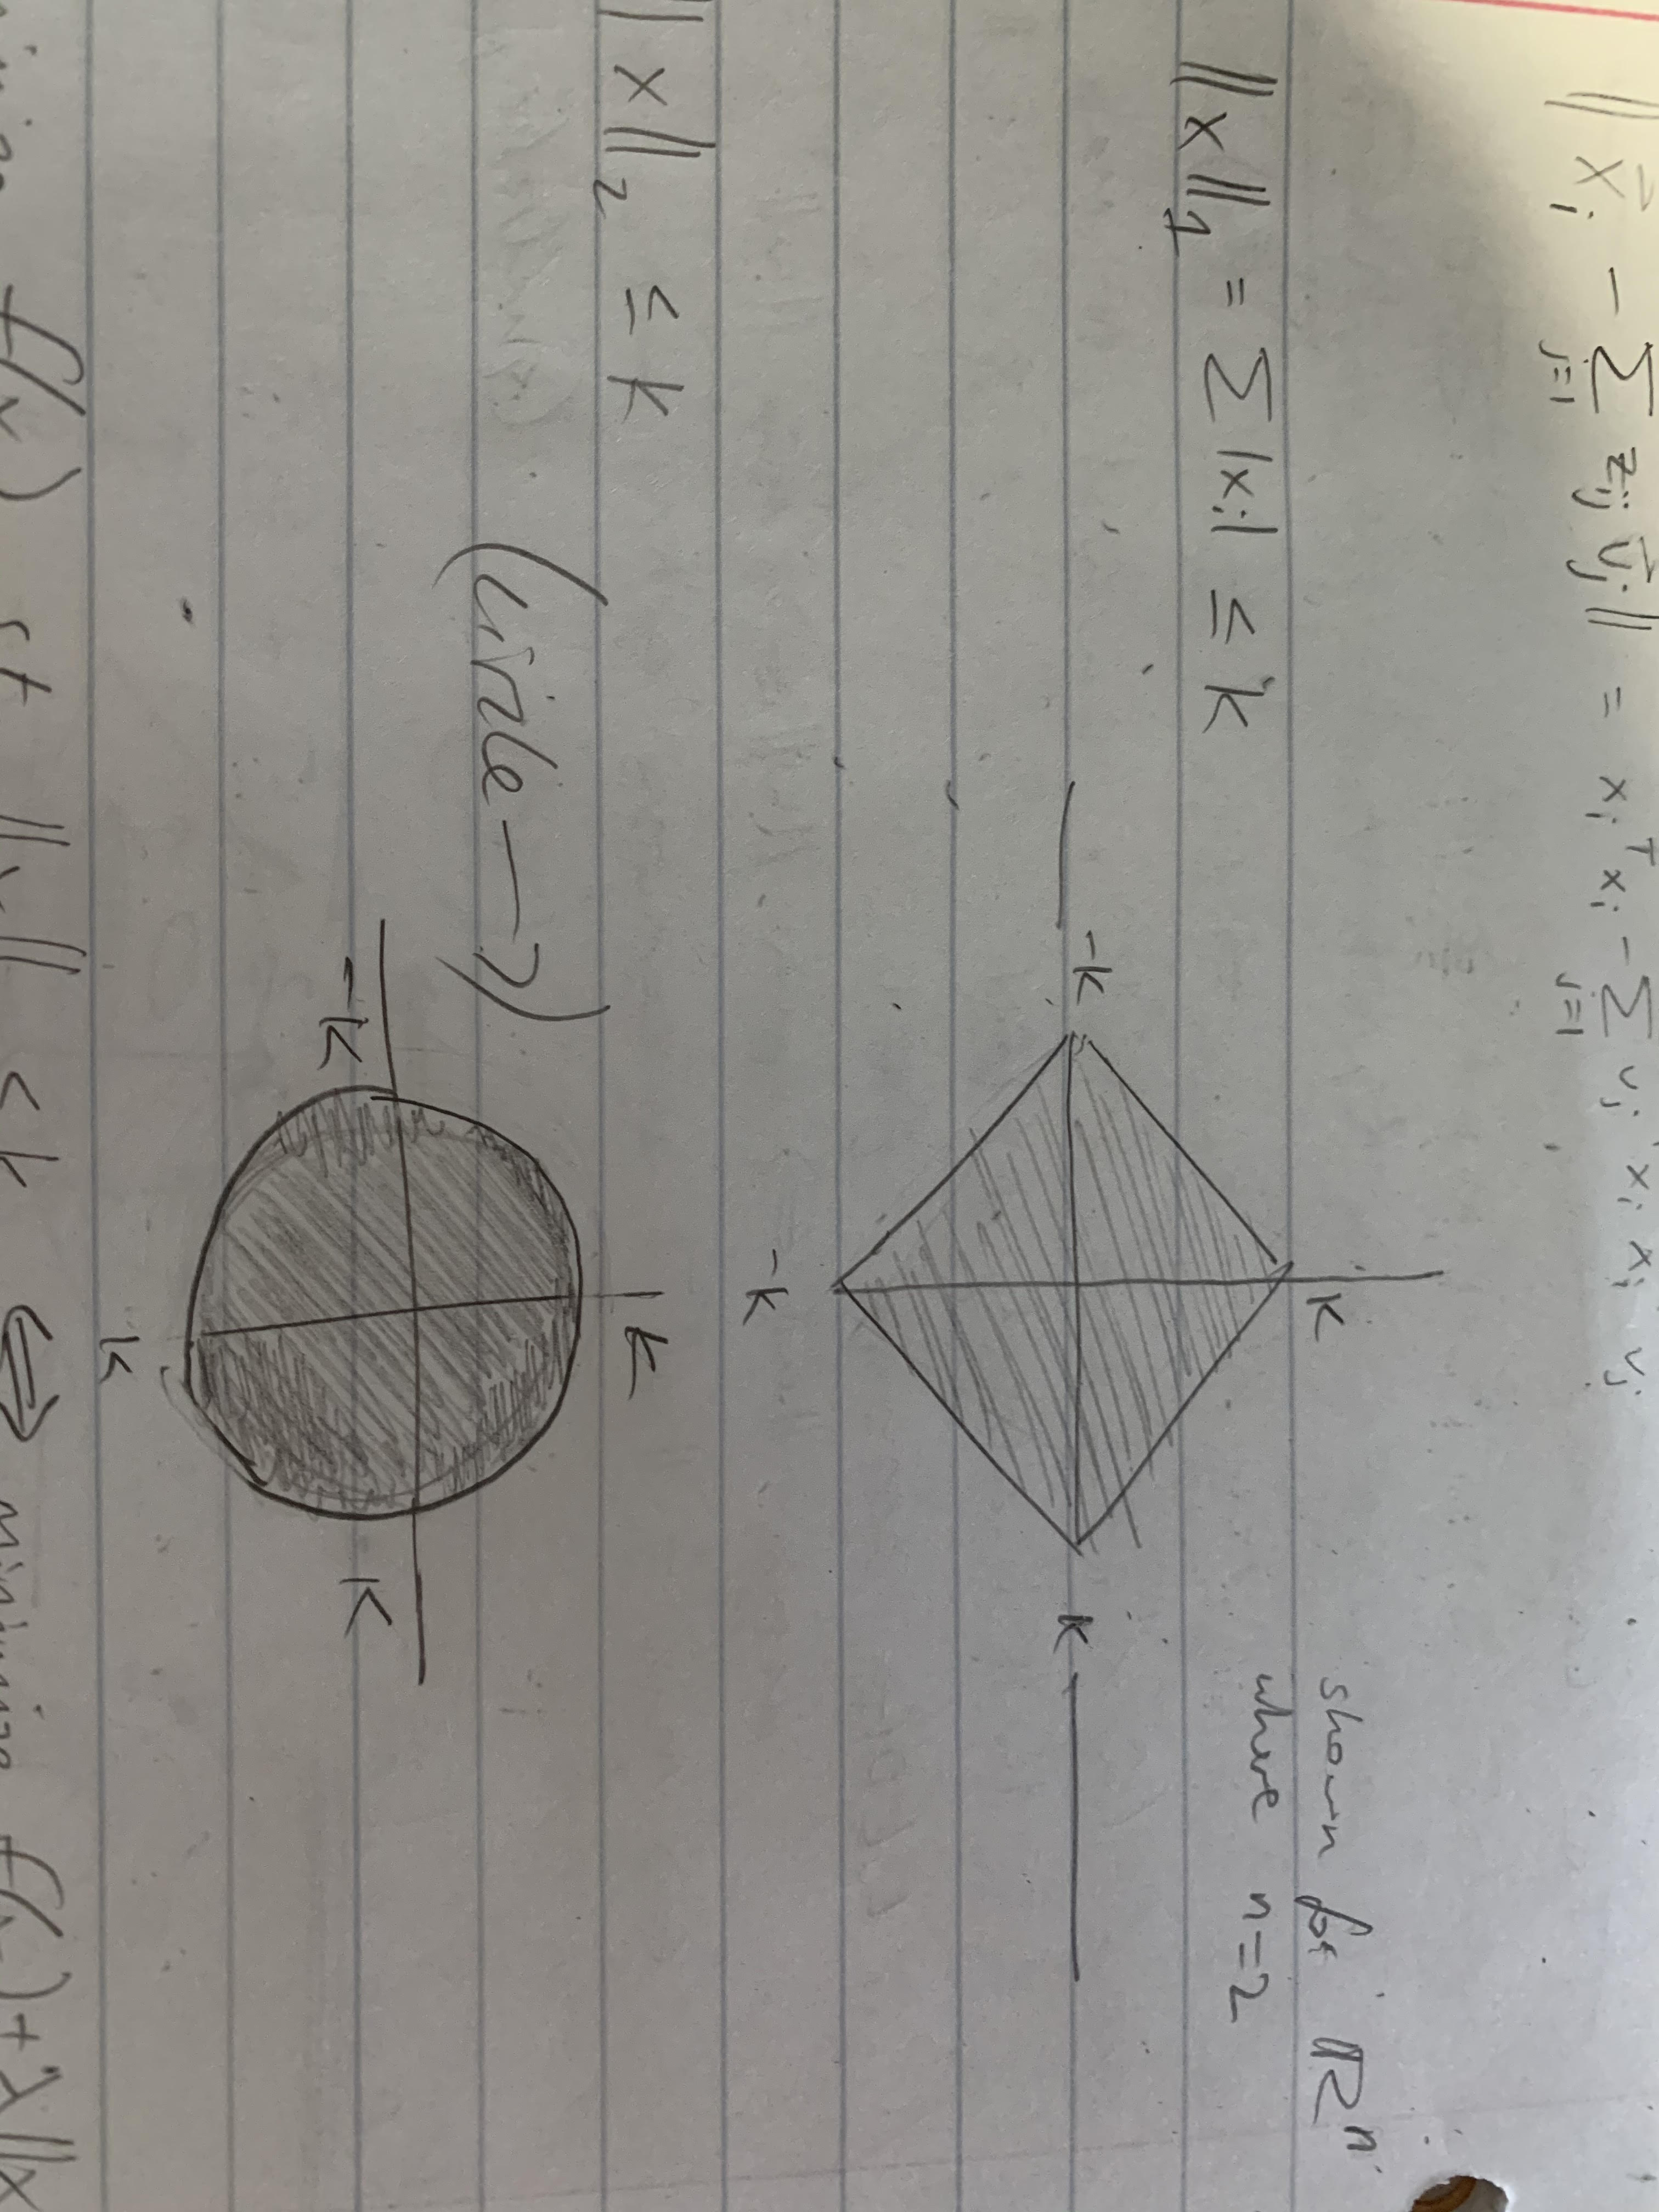
\includegraphics[width=0.8\textwidth, angle=90]{norm}

    With the constraint $\|\xx\|_p \leq k$, the Lagrangian is $L(\xx, \lambda) = f(\xx) + \lambda \|\xx\|_p$

    The derivative $\frac{d\|\xx\|_p}{d\xx} = \frac{\sum |\xx_i|^{p-1} \cdot \text{sgn} \xx_i}{\|\xx\|_p^{p-1}}$.

    When $p=1$, if $x_i = 0$ then the contribution to the derivative is 0. If $x_i < 0$, the contribution is negative, and if $x_i > 0$, the contribution is positive, so the $x_i$ will be 'squeezed' towards 0 when minimizing $\frac{d\|\xx\|_p}{d\xx}$.

    When $p=2$, the contributions are proportional to both the sign of $x_i$ and their magnitude so the minimizing $\xx$ is less sparse.

    (got help from https://stats.stackexchange.com/questions/45643/why-l1-norm-for-sparse-models )
\end{solution}
\newpage



\begin{problem}[Extra Credit]
\textbf{(Lasso)} Show that placing an equal zero-mean Laplace prior on each element of the weights $\thetab$
of a model is equivelent to $\ell_1$ regularization in the Maximum-a-Posteriori estimate
\begin{align*}
    \text{maximize: } & \PP(\thetab | \Dc) = \frac{\PP(\Dc | \thetab)\PP(\thetab)}{\PP(\Dc)}.
\end{align*}
Note the form of the Laplace distribution is
\[
    \mathrm{Lap}(x|\mu,b) = \frac{1}{2b}\exp\left(-\frac{|x-\mu|}{b}\right)
\]
where $\mu$ is the location parameter and $b>0$ controls the variance. Draw (by hand) and compare the density
$\mathrm{Lap}(x|0,1)$ and the standard normal $\Nc(x|0,1)$ and suggest why this would
lead to sparser solutions than a Gaussian prior on each elements of the weights
(which correspond to $\ell_2$ regularization).
\end{problem}
\begin{solution}
\vfill
\end{solution}

\end{document}
